%% —-----------------------------------------------------------
%% sbcreviews-pt.tex
%% Template para SBC Reviews 
%% (https://journals-sol.sbc.org.br/index.php/reviews/) 
%% 
%% Esta versão do template para a SBC Reviews inclui algumas
%% modificações sobre o template original da REIC
%% (https://journals-sol.sbc.org.br/index.php/reic)
%%
%% Licença CC BY 4.0 (https://creativecommons.org/licenses/by/4.0/)
%% Sociedade Brasileira de Computação.

\documentclass[portuguese]{sbcreviews-2025}%
\usepackage[misc,geometry]{ifsym} 

%\usepackage{graphicx} % carregada dentro da classe
%\usepackage{fontspec} % carregada dentro da classe
%\usepackage{fontawesome} % carregada dentro da classe
%\usepackage{color} % carregada dentro da classe
%\usepackage{hyperref} % carregada dentro da classe

\usepackage{aas_macros}
\usepackage[bottom]{footmisc}

\usepackage{tabularray}
% O pacote tabularray torna o uso dos pacotes abaixo desnecessarios.
%\usepackage{supertabular}
%\usepackage{multicol}
%\usepackage{multirow}

\usepackage{afterpage}
\usepackage{url}
\usepackage{pifont}

\setcitestyle{square}

\definecolor{engtitle}{rgb}{0.5,0.5,0.5}
\definecolor{orcidlogo}{rgb}{0.37,0.48,0.13}
\definecolor{unilogo}{rgb}{0.16, 0.26, 0.58}
\definecolor{maillogo}{rgb}{0.58, 0.16, 0.26}
\definecolor{darkblue}{rgb}{0.0,0.0,0.0}
\hypersetup{colorlinks,breaklinks,
            linkcolor=darkblue,urlcolor=darkblue,
            anchorcolor=darkblue,citecolor=darkblue}
%\hypersetup{colorlinks,citecolor=blue,linkcolor=blue,urlcolor=blue}
% We disable hyperlinks by default with this line, to avoid the error "\pdfendlink ended up in different nesting level" while writing.

\jid{ROCS}
\jtitle{SBC Computing Reviews, 202X, XX:1}
\issn{2966-3938}
\doi{10.5753/rocs.202X.XXXXXX}
\copyrightstatement{This work is licensed under a Creative Commons Attribution 4.0 International License}
\jyear{202X}

\category{Revisão da Literatura}
\title[Template da SBC Reviews 2025 para artigos em português]{Apresentação do template da SBC Reviews 2025 - Versão para artigos em português}
\engtitle{\textcolor{engtitle}{Presenting the SBC Reviews 2025 template - Version for papers in Portuguese}}

%THE ORCID IS MANDATORY FOR EACH AUTHOR
\author[Silva et al. 202X]{
\affil{\textbf{João Silva}~\orcidlink{0000-0000-0000-0000}~\textcolor{blue}{\faEnvelope}~~[{Universidade Federal}~|\href{mailto: ...}{~{\textit{...@...br}}}~]}

\affil{\textbf{Maria Santos}~\orcidlink{0000-0000-0000-0000}~[{Universidade Federal}~|\href{mailto: ...}{~{\textit{...@...br}}}~]}

\affil{\textbf{Ana Silva }~\orcidlink{0000-0000-0000-0000}~[{Universidade Federal}~|\href{mailto: ...}{~{\textit{...@...br}}}~]}

\affil{\textbf{José Santos}~\orcidlink{0000-0000-0000-0000}~[{Universidade Federal}~|\href{mailto: ...}{~{\textit{...@...br}}}~]}

}

\begin{document}

\begin{frontmatter}

\maketitle

\begin{mail}
Instituto ..., Universidade ..., Endereço, Cidade, Estado, CEP, Brasil. 
\end{mail}


\begin{abstract-pt}
Este texto, em formato de artigo científico, tem por objetivo apresentar o novo modelo para artigos da SBC, descrevendo suas principais características e explicando como deve ser utilizado. Esta versão, mais especificamente, deve ser utilizada exclusivamente para artigos escritos em português que serão publicados em alguma série de anais de eventos na SBC OpenLib. O resumo em português, como pode-se notar neste exemplo, deve vir antes do resumo em inglês (abstract) e ter entre 500 e 750 palavras.
\end{abstract-pt}

\begin{abstract-en}
This text, formatted as a scientific article, aims to present the new SBC paper template, describing its main features and explaining how it should be used. This version, more specifically, should be used exclusively for articles written in Portuguese that will be published in any event proceeding series at SBC OpenLib. The abstract in Portuguese, as you can see in this example, must be before the abstract in English and must have between 500 and 750 words.
\end{abstract-en}

\begin{pchaves}
Anais de evento, Modelo, SBC OpenLib, Indexação
\end{pchaves}

\begin{keywords}
Proceedings, Template, SBC OpenLib, Indexing
\end{keywords}

\begin{dates}
% This information will be provided by the editor before publishing the paper
\noindent{\sffamily\textbf{Recebido/Received:}} DD Month YYYY~~~$\bullet$~~~
{\sffamily\textbf{Aceito/Accepted:}} DD Month YYYY~~~$\bullet$~~~
{\sffamily\textbf{Publicado/Published:}} DD Month YYYY
\end{dates}


%\begin{license}
%Published under the Creative Commons Attribution 4.0 International Public License (CC BY 4.0)
%\end{license}

\end{frontmatter}
\section{Escopo, método e critério de confiança}
\label{sec:escopo}

Este relatório reconstrói, com prioridade epistemológica explícita, o conteúdo dos arquivos \texttt{4.tracado\_de\_raios.pdf}, \texttt{5.tracado\_de\_raios2.pdf} e \texttt{6.estrutura\_aceleracao.pdf}, usando os resumos em \path{materiais/traçado_de_raios/*.md} apenas como apoio de leitura e o código em \path{src/ray_tracing_2/} como evidência de implementação. A documentação em \path{docs/*.md} foi usada apenas como apoio secundário de estrutura e nunca como autoridade teórica principal.

O objetivo não é apenas resumir os slides, mas separar três camadas que frequentemente se confundem em relatórios de implementação:

\begin{enumerate}
    \item a formulação geométrica e física apresentada nos slides;
    \item a tradução algorítmica que o repositório efetivamente materializa;
    \item as lacunas entre o conteúdo didático e a implementação entregue.
\end{enumerate}

Como fonte externa, foi usado somente o conteúdo de PBRT 4e permitido pelo enunciado, principalmente os trechos sobre câmera projetiva, teoria de amostragem, reflexão e transmissão especular, transmitância, luzes de área, caixas envolventes e BVHs. Em particular, foram úteis: PBRT 4e \S\S 1.2, 3.5, 3.7, 5.2, 8.1, 8.5, 9.3, 9.5, 11.2, 12.4 e 7.3.

\section{Plano Consolidado do Relatório}
\label{sec:plano-relatorio}

\begin{enumerate}
    \item Reconstituir o núcleo do Slide 4: raio paramétrico, interseções básicas, câmera pinhole, Phong, luz pontual e sombra dura.
    \item Explicitar a base de álgebra linear do projeto: mudança de base, espaços local/global, vetores normais e transformações homogêneas.
    \item Descrever as extensões do Slide 5: supersampling, instanciação, luz de área, AABB/slabs, recursão, Fresnel-Schlick, Snell, reflexão interna total e Beer-Lambert.
    \item Mostrar como a implementação transforma o teste de sombra binário do Slide 4 em transmitância acumulada no Slide 5.
    \item Reconstituir o Slide 6 em três níveis: triângulo isolado, malha triangulada e estruturas de aceleração.
    \item Distinguir com precisão o que o repositório implementa do que o Slide 6 descreve apenas teoricamente.
    \item Ancorar cada bloco com referências de páginas dos slides e linhas do código atual.
    \item Fechar com uma validação experimental breve, usando renderizações já existentes no repositório.
    \item Consolidar, ao fim, as limitações atuais da implementação frente aos materiais da disciplina e ao escopo do enunciado principal.
\end{enumerate}

\section{Slide 4: Núcleo Geométrico e Fotométrico do Traçador}
\label{sec:slide4}

\subsection{Conceitos Estruturantes do Slide 4}
\label{sec:slide4-conceitos}

O Slide 4 organiza-se em torno de um conjunto pequeno de conceitos que estrutura todo o traçador de raios.

\begin{enumerate}
    \item \textbf{Raio paramétrico e visibilidade (pp. 7-9).} A formulação $\mathbf{r}(t)=\mathbf{o}+t\,\hat{\mathbf{d}}$ reduz a linha de visada a uma reta orientada; $t$ funciona como distância assinada ou paramétrica ao longo do feixe, e a visibilidade do ponto observado é determinada pelo menor $t>0$ compatível com uma superfície.
    \item \textbf{Interseções analíticas e controle numérico (pp. 10-18).} O plano é descrito por $(\mathbf{x}-\mathbf{p}_0)\cdot\hat{\mathbf{n}}=0$, enquanto a esfera leva à quadrática $at^2+bt+c=0$, cujo discriminante $\Delta$ classifica ausência, tangência ou dupla interseção; do ponto de vista computacional, essa geometria analítica só é robusta quando acompanhada por um critério de tolerância $\varepsilon$ para rejeitar paralelismos numéricos e auto-interseções.
    \item \textbf{Câmera pinhole, filme e mudança de base (pp. 19-39).} A câmera é construída por uma base ortonormal $(\hat{\mathbf{u}},\hat{\mathbf{v}},\hat{\mathbf{w}})$ e pela geometria do filme, com $\Delta v = f\tan(\theta/2)$ e $\Delta u = \Delta v\,(w/h)$; em síntese, esse bloco combina geometria projetiva com mudança de base entre espaço da câmera e espaço global.
    \item \textbf{Iluminação local e fotometria simplificada (pp. 40-43).} O modelo local de Phong combina a componente difusa lambertiana $\max(0,\hat{\mathbf{n}}\cdot\hat{\mathbf{l}})$ com a componente especular $\max(0,\hat{\mathbf{r}}\cdot\hat{\mathbf{v}})^s$; fisicamente, trata-se de um modelo local e fenomenológico, útil para capturar dependência angular sem resolver transporte global de luz.
    \item \textbf{Organização algorítmica da cena, sombras e luz ambiente (pp. 44-55).} O pipeline de \emph{closest hit} seleciona a primeira interseção visível, o raio de sombra transforma a iluminação direta em um teste de visibilidade até a fonte, e o termo ambiente $m_{amb}\,l_{amb}$ fecha o modelo como aproximação empírica da iluminação indireta ausente.
\end{enumerate}

Esses conceitos explicam por que as subseções seguintes podem ser lidas como desdobramentos detalhados do mesmo núcleo conceitual.

\subsection{Raio paramétrico, visibilidade e registro de interseção}
\label{sec:slide4-raio}

O ponto de partida do Slide 4 é a modelagem do raio por

\[
\mathbf{r}(t)=\mathbf{o}+t\,\hat{\mathbf{d}},\qquad t\ge 0,
\]

em que $\mathbf{o}$ é a origem, $\hat{\mathbf{d}}$ é a direção normalizada e $t$ parametriza a posição ao longo do feixe. Em ótica geométrica, essa formulação abstrai a propagação retilínea da luz em meios homogêneos; em computação gráfica, ela converte o problema de visibilidade em um problema de encontrar o menor $t$ positivo compatível com uma superfície. Nos slides, isso aparece como o elo entre câmera, interseção e sombreamento local, particularmente na dedução do raio paramétrico e na interpretação física de $t$ como distância assinada ao longo da trajetória (\texttt{4.tracado\_de\_raios.pdf}, pp. 7-9).

O repositório segue exatamente essa organização. O raio é carregado por \texttt{Ray}, enquanto \texttt{Hit} armazena a melhor interseção conhecida até o momento e também codifica \texttt{front\_face} e \texttt{backfacing}. Essa distinção, que no Slide 4 serve para consistência geométrica da normal, torna-se decisiva no Slide 5 para distinguir entrada e saída de meios refrativos. A rotina \texttt{Scene.compute\_intersection()} preserva o padrão clássico de \emph{closest hit}: percorre os objetos, atualiza um único registro acumulador e retorna apenas a interseção frontal mais próxima.

\noindent\textbf{Rastreabilidade no código.} \path{src/ray_tracing_2/hit.py} (\texttt{Hit}, l. 11; \texttt{set\_face\_normal()}, l. 25), \path{src/ray_tracing_2/scene.py} (\texttt{compute\_intersection()}, l. 24; \texttt{trace\_ray()}, l. 102).

PBRT 4e de apoio: \S\S 1.2 e 3.5.

\subsection{Interseções básicas: plano, esfera e controle numérico de $\varepsilon$}
\label{sec:slide4-intersecoes}

Nos slides, o plano é descrito pela equação implícita

\[
(\mathbf{x}-\mathbf{p}_0)\cdot\hat{\mathbf{n}}=0,
\]

e a substituição de $\mathbf{r}(t)$ produz a solução linear

\[
t=\frac{(\mathbf{p}_0-\mathbf{o})\cdot\hat{\mathbf{n}}}{\hat{\mathbf{d}}\cdot\hat{\mathbf{n}}},
\]

exatamente como discutido nas páginas de interseção raio-plano (\texttt{4.tracado\_de\_raios.pdf}, pp. 10-13). A esfera, por sua vez, impõe

\[
\lVert\mathbf{x}-\mathbf{c}\rVert^2-r^2=0,
\]

que, após substituição do raio, gera uma quadrática $at^2+bt+c=0$ cujo discriminante $\Delta=b^2-4ac$ decide ausência, tangência ou dupla interseção (\texttt{4.tracado\_de\_raios.pdf}, pp. 14-18). Em ambos os casos, o aspecto fisicamente relevante é o mesmo: o que interessa para a câmera é a menor raiz positiva. O aspecto numericamente relevante também é comum: deve-se rejeitar soluções com $t$ demasiado pequeno para evitar reinterseção artificial da própria superfície.

O código espelha esse raciocínio. \texttt{Plane.intersect()} resolve o plano por produto escalar; \texttt{Sphere.intersect()} resolve a quadrática e guarda a menor raiz positiva; \texttt{Scene.offset\_point()} empurra a origem dos raios secundários ao longo da normal geométrica com \texttt{ray\_epsilon = 0.001}, evitando \emph{shadow acne} em sombra, reflexão e refração. O Slide 4 apresenta essa ideia como tolerância numérica; o repositório a aplica de forma centralizada, o que é arquiteturalmente melhor do que espalhar pequenos limiares por todos os materiais.

\noindent\textbf{Rastreabilidade no código.} \path{src/ray_tracing_2/shape.py} (\texttt{Sphere}, l. 17; \texttt{Sphere.intersect()}, l. 23; \texttt{Plane}, l. 54; \texttt{Plane.intersect()}, l. 60), \path{src/ray_tracing_2/scene.py} (\texttt{offset\_point()}, l. 33).

PBRT 4e de apoio: \S 1.2.

\subsection{Câmera pinhole, filme e espaços de coordenadas}
\label{sec:slide4-camera}

O Slide 4 reconstrói o modelo pinhole por uma base ortonormal de câmera, usando \texttt{eye}, \texttt{center} e \texttt{up} para montar os eixos locais (pp. 19-23), e em seguida projeta amostras do pixel sobre o plano de imagem (pp. 24-29), antes de explicitar a mudança entre espaço de câmera e espaço global (pp. 31-39) (\texttt{4.tracado\_de\_raios.pdf}). A formulação algébrica é a de uma mudança de base: do espaço local da câmera para o espaço global da cena. Em uma formulação clássica, isso aparece como matriz de visualização, sua inversa e projeção perspectiva parametrizada por campo de visão, aspecto e distância ao plano de imagem.

No código, a ideia é a mesma, mas a implementação é condensada: \texttt{Camera.\_\_init\_\_()} usa \texttt{glm.lookAt()} para obter a transformação de visualização e armazena sua inversa em \texttt{inv\_view}. A geração do raio em \texttt{generate\_ray()} monta o ponto do pixel em espaço de câmera a partir de coordenadas normalizadas e da relação trigonométrica

\[
\Delta v = f\tan\left(\frac{\theta}{2}\right),\qquad \Delta u = \Delta v\,\frac{w}{h},
\]

que é precisamente a síntese entre geometria projetiva e semelhança de triângulos apresentada nos slides (pp. 24-29), e depois transforma esse ponto para o espaço global (pp. 31-39). O comentário recém-ajustado em \texttt{camera.py} deixa explícita uma nuance importante: \texttt{focal\_distance} aqui é distância geométrica ao plano de projeção no modelo pinhole, não distância focal de lente fina nem parâmetro de profundidade de campo. Esse detalhe é essencial para não projetar sobre o código uma física que ele não implementa.

Essa distinção também define uma limitação importante do projeto: todos os raios primários partem de um único centro ótico, sem abertura finita, círculo de confusão ou profundidade de campo. Portanto, o antialiasing implementado depois no Slide 5 altera a estratégia de amostragem do pixel, mas não muda o modelo óptico de formação de imagem.

Em \texttt{film.py}, \texttt{get\_sample()} e \texttt{render()} deixam claro que a imagem final é construída como média de amostras por pixel. Mesmo quando o caso básico usa apenas uma amostra central, a interface já está preparada para supersampling estocástico.

\noindent\textbf{Rastreabilidade no código.} \path{src/ray_tracing_2/camera.py} (\texttt{Camera}, l. 6; \texttt{\_\_init\_\_()}, l. 7; \texttt{generate\_ray()}, l. 23), \path{src/ray_tracing_2/film.py} (\texttt{Film}, l. 20; \texttt{get\_sample()}, l. 54; \texttt{render()}, l. 108), \path{src/ray_tracing_2/main.py} (\texttt{render()}, l. 25).

PBRT 4e de apoio: \S 5.2.

\subsection{Phong, luz pontual, termo ambiente e sombra dura}
\label{sec:slide4-phong}

O Slide 4 fecha o núcleo do renderizador com o modelo local de Phong, isto é, uma soma de termo ambiente, componente difusa lambertiana e componente especular dependente do vetor refletido (\texttt{4.tracado\_de\_raios.pdf}, pp. 40-43 e 54-55). Em termos físicos, esse modelo não é um BRDF rigoroso, mas é uma aproximação útil: o termo difuso usa o fator $\max(0,\hat{\mathbf{n}}\cdot\hat{\mathbf{l}})$; o termo especular usa um pico angular em função de $\max(0,\hat{\mathbf{r}}\cdot\hat{\mathbf{v}})^s$; a sombra dura decorre de um teste binário de visibilidade entre o ponto sombreado e a fonte (\texttt{4.tracado\_de\_raios.pdf}, pp. 51-53). Em particular, as páginas 40-43 articulam a síntese física mínima do projeto: incidência luminosa, orientação local de normal e dependência angular da resposta da superfície.

\texttt{PhongMaterial.direct\_lighting()} implementa exatamente esse cálculo. Para cada luz, o código obtém radiância incidente e direção via \texttt{sample\_radiance()}, soma o termo difuso e depois o termo especular. \texttt{Scene.transmittance()} faz o papel do raio de sombra, mas já em uma forma mais geral: para meios opacos, ele reduz-se ao teste binário do Slide 4; para meios transparentes, ele vira um produto acumulado de transmitâncias, o que antecipa o Slide 5.

Há, contudo, uma nuance importante entre a física dos slides e a convenção da implementação: os slides apresentam a lei usual de decaimento geométrico de uma fonte pontual, proporcional a $1/r^2$, mas \texttt{PointLight.radiance()} não aplica esse fator. O comentário do código explicita a razão: o projeto preserva a convenção do enunciado em que \texttt{power} é tratado como radiância constante da fonte. Isso não é um erro, mas uma simplificação de modelagem que precisa ser declarada no relatório para evitar falsa equivalência com uma formulação radiométrica completa.

\noindent\textbf{Rastreabilidade no código.} \path{src/ray_tracing_2/light.py} (\texttt{PointLight}, l. 42; \texttt{PointLight.radiance()}, l. 46), \path{src/ray_tracing_2/material.py} (\texttt{PhongMaterial}, l. 37; \texttt{direct\_lighting()}, l. 45; \texttt{eval()}, l. 72), \path{src/ray_tracing_2/scene.py} (\texttt{transmittance()}, l. 48), \path{src/ray_tracing_2/main.py} (\texttt{Sphere}, l. 54; \texttt{Plane}, l. 55; \texttt{PointLight}, l. 59).

PBRT 4e de apoio: \S 1.2.

\subsection{Quadro de aderência entre Slide 4 e implementação}
\label{sec:slide4-quadro}

\begin{table*}[!ht]
\caption{Quadro de aderência entre o Slide 4 e a implementação atual.}
\label{tab:slide4-aderencia}
\centering
\begin{tblr}{
width=\textwidth,
colspec={Q[l,wd=0.24\textwidth] Q[l,wd=0.17\textwidth] Q[l,wd=0.50\textwidth]},
row{1}={font=\bfseries},
rows={valign=t}
}
Conceito do Slide 4 & Situação no repositório & Evidência \\
Raio paramétrico e registro de hit & Implementado & \texttt{Ray}; \texttt{Hit}; \texttt{Scene.compute\_intersection()} \\
Interseção raio-plano & Implementado & \texttt{Plane.intersect()} \\
Interseção raio-esfera & Implementado & \texttt{Sphere.intersect()} \\
Tolerância numérica para evitar auto-interseção & Implementado & \texttt{Scene.offset\_point()}; limiar positivo nas interseções \\
Câmera pinhole e geração de raios primários & Implementado & \texttt{Camera.\_\_init\_\_()}; \texttt{Camera.generate\_ray()} \\
Mudança de base entre espaço da câmera e espaço global & Implementado & \texttt{glm.lookAt()} + \texttt{inv\_view} em \texttt{Camera} \\
Modelo local de Phong com ambiente, difusa e especular & Implementado & \texttt{PhongMaterial.direct\_lighting()}; \texttt{PhongMaterial.eval()} \\
Sombra dura por teste de visibilidade & Implementado com generalização & \texttt{Scene.transmittance()} reduz-se ao caso binário para opacos e estende o slide para transparentes \\
Luz pontual com síntese radiométrica do slide & Implementado com simplificação & \texttt{PointLight.radiance()} usa a convenção do enunciado sem queda explícita por $1/r^2$ \\
Estrutura algorítmica básica câmera-hit-sombreamento & Implementado & \texttt{Film.render()}; \texttt{Camera.generate\_ray()}; \texttt{Scene.trace\_ray()} \\
\end{tblr}
\end{table*}

O quadro mostra que o núcleo conceitual do Slide 4 está efetivamente materializado no repositório, mas com duas qualificações importantes: a luz pontual segue a convenção simplificada do enunciado, e o teste de sombra já aparece no código em forma mais geral do que a apresentada no bloco introdutório dos slides.
  
\section{Sobre a SBC Reviews}

Os tópicos de interesse incluem, mas não estão limitados a:

\begin{itemize}
\item Algoritmos, Combinatória e Otimização
\item Inteligência Artificial
\item Sistemas Colaborativos
\item Biologia Computacional
\item Inteligência Computacional
\item Computação Gráfica e Processamento de Imagens
\item Redes de Computadores e Sistemas Distribuídos
\item Ontologias Computacionais
\item Engenharia de Sistemas Computacionais
\item Computação Aplicada à Saúde
\item Educação em Computação
\item Modelagem Conceitual
\item Bancos de Dados
\item Projeto de Circuitos e Sistemas Integrados
\item Jogos Digitais e Entretenimento
\item Sistemas Tolerantes a Falhas
\item Métodos Formais
\item Geoinformática
\item Computação Verde
\item Arquitetura e Processamento de Computadores de Alto Desempenho
\item Aspectos Humanos e Sociais na Computação
\item Interação Humano-Computador
\item Informática na Educação
\item Segurança da Informação e de Sistemas Computacionais
\item Informação Sistemas
\item Sistemas Multimídia e Web
\item Computação Musical
\item Processamento de Linguagem Natural
\item Linguagens de Programação
\item Robótica
\item Engenharia de Software
\item Realidade Virtual
\end{itemize}

Os dois pacotes \texttt{fontenc} e \texttt{fontspec} pertencem a ``universos'' distintos e não devem ser ambos incluídos no mesmo preâmbulo sob a pena de conflitos.

O pacote \texttt{fontspec} lida com o universo dos fontes Truetype e/ou Opentype. 
A distribuição TeXlive---a qual é usada pelo Overleaf---instala uma vasta gama de fontes: por exemplo, o \textbf{TeX Gyre Termes} é o equivalente livre e gratuito do fonte \textbf{Times New Roman}. 

Obs: para os engines xetex e luatex não é obrigatório realizar a inclusão do pacote \texttt{fontspec}. A omissão faz o engine assumir valores default para fonte e suas propriedades.

Para o engine pdftex, o pacote a ser incluido deveria ser o \textbf{fontenc}. 
A inclusão desse pacote faz com que o engine leia arquivos de definição, e outros associados e com isso executa uma ligação ``estrita'' ao fonte.  

\begin{table}[!ht]
\caption{Exemplo de legenda de tabela.}
\centering
\begin{tabular}{@{}cc@{}}
\hline\hline
Dimensão & Classificação\\
\hline%
 1  & 0.6232 \\
 2  & 0.9635 \\ 
 3  & 0.9724 \\ 
 4  & 0.9690 \\ 
 5  & 0.9840 \\ 
 6  & 0.9842 \\ 
 7  & 0.9873 \\ 
 8  & 0.9884 \\
 9  & 0.9873 \\ 
 10 & 0.9898 \\ 
 11 & 0.9914 \\
\hline\hline
\end{tabular}
\label{tab1}
\end{table}

Lorem ipsum dolor sit amet, consectetur adipiscing elit, sed do eiusmod tempor incididunt ut labore et dolore magna aliqua. Ut enim ad minim veniam, quis nostrud exercitation ullamco laboris nisi ut aliquip ex ea commodo consequat. Duis aute irure dolor in reprehenderit in voluptate velit esse cillum dolore eu fugiat nulla pariatur. Excepteur sint occaecat cupidatat non proident, sunt in culpa qui officia deserunt mollit anim id est laborum (see \textbf{ Table~\ref{tab1}}). 
Assim, recomendamos fortemente o uso do pacote \texttt{tabularray}. 

\begin{table}[!ht]
\caption{Exemplo de legenda de tabela.}
\centering
\begin{tblr}{%
columns={c},
row{even}={gray9},
row{1}={bg=red!10, font=\bfseries}
}
\hline
Dimensão & Classificação\\
\hline%
 1  & 0.6 \\
 2  & 0.963 \\ 
 3  & 0.97 \\ 
 4  & 0.9690 \\ 
 5  & 0.9840 \\ 
 6  & 0.98423 \\ 
 7  & 0.9873 \\ 
 8  & 0.9884 \\
 9  & 0.9873 \\ 
 10 & 0.9898 \\ 
 11 & 0.991 \\
\end{tblr}
\label{tab1-1}
\end{table}

Lorem ipsum dolor sit amet, consectetur adipiscing elit, sed do eiusmod tempor incididunt ut labore et dolore magna aliqua. Ut enim ad minim veniam, quis nostrud exercitation ullamco laboris nisi ut aliquip ex ea commodo consequat. Duis aute irure dolor in reprehenderit in voluptate velit esse cillum dolore eu fugiat nulla pariatur. Excepteur sint occaecat cupidatat non proident, sunt in culpa qui officia deserunt mollit anim id est laborum \citep{ref3}, dolor sit amet, consectetur adipiscing elit, sed do eiusmod tempor incididunt ut labore et dolore magna aliqua. Ut enim ad minim veniam, quis nostrud exercitation ullamco laboris nisi ut aliquip ex ea commodo consequat.

Lorem ipsum dolor sit amet, consectetur adipiscing elit, sed do eiusmod tempor incididunt ut labore et dolore magna aliqua. Ut enim ad minim veniam, quis nostrud exercitation ullamco laboris nisi ut aliquip ex ea commodo consequat~\citep{ref4}.

\subsection{Modelo de Publicação}

A SBC Reviews adota o modelo de Publicação Contínua, o que significa que os artigos são publicados imediatamente após a aceitação, sem esperar pela compilação de uma edição completa. Essa abordagem acelera a disseminação e a disponibilidade de descobertas científicas, beneficiando pesquisadores, estudantes, leitores, editoras e agências de fomento, promovendo rapidez e acesso oportuno a pesquisas de alta qualidade para leitura e citação.

\subsection{Acesso Aberto Diamante}

A SBC Reviews é de acesso aberto e gratuito para autores e leitores. Todos os artigos publicados pela SBC Reviews são disponibilizados online de forma gratuita e permanente imediatamente após a publicação, sem taxas de assinatura ou barreiras de registro. Acreditamos que a política adotada elimina barreiras econômicas e geográficas, promove a democratização global e acelera o progresso da pesquisa.

\subsection{Aviso de Direitos Autorais}
Os autores que publicam na SBC Reviews mantêm os direitos autorais de seus artigos e autorizam a SBC a publicá-los sob os termos da Licença Pública Internacional Creative Commons Atribuição 4.0 (CC BY 4.0). Assim, os autores ou terceiros podem reproduzir ou distribuir, no todo ou em parte, conteúdo extraído dos artigos publicados, na íntegra, adaptado ou remixado, desde que sejam atribuídos os devidos créditos aos autores originais e à publicação original.

\section{Submissões}

\subsection{Checklist de Preparação para Submissão}

Como parte do processo de submissão, os autores devem verificar a conformidade de sua submissão com todos os itens a seguir. As submissões poderão ser devolvidas aos autores que não seguirem estas diretrizes.

\section{Revisões de Literatura}

Revisões de literatura são estudos retrospectivos e observacionais.
A SBC Reviews publica revisões de literatura em áreas de pesquisa em Computação, incluindo, entre outros, os seguintes tipos de revisão:

\textbf{Revisões sistemáticas de literatura} são revisões rigorosas e abrangentes que visam responder a uma questão de pesquisa específica e focada, avaliando e sintetizando criticamente todos os estudos de pesquisa originais relevantes. Se métodos estatísticos forem usados para combinar dados quantitativos de vários estudos, trata-se de um estudo de Meta-Análise.

\textbf{Revisões multivocais da literatura} são um tipo de RSL que incorpora tanto literatura formal revisada por pares (como artigos de periódicos e trabalhos de conferências) quanto literatura cinzenta. A literatura cinzenta inclui materiais como relatórios técnicos, postagens em blogs e apresentações em conferências, que podem não ser formalmente publicados ou revisados por pares.

\textbf{Revisões de escopo} abordam questões de pesquisa mais amplas e exploratórias para mapear a extensão, o alcance e a natureza da pesquisa sobre um tópico específico. Entre outros objetivos, as revisões de escopo ajudam a determinar se uma revisão sistemática da literatura é necessária.

\textbf{Mapeamentos sistemáticos da literatura} concentram-se na categorização e quantificação da literatura existente para fornecer uma visão geral da atividade de pesquisa em um subcampo.

O periódico SBC Reviews também avalia submissões de revisões de literatura que abordam avaliações de progresso e/ou avaliações críticas relevantes para subcampos específicos.

\section{Exemplo de Título Nível 1 (Seção)}
Lorem ipsum dolor sit amet, consectetur adipiscing elit, sed do eiusmod tempor incididunt ut labore et dolore magna aliqua. Ut enim ad minim veniam, quis nostrud exercitation ullamco laboris nisi ut aliquip ex ea commodo consequat. Duis aute irure dolor in reprehenderit in voluptate velit esse cillum dolore eu fugiat nulla pariatur. Excepteur sint occaecat cupidatat non proident, sunt in culpa qui officia deserunt mollit anim id est laborum. Lorem ipsum dolor sit amet, consectetur adipiscing elit, sed do eiusmod tempor incididunt ut labore et dolore magna aliqua. Ut enim ad minim veniam, quis nostrud exercitation ullamco laboris nisi ut aliquip ex ea commodo consequat. Duis aute irure dolor in reprehenderit in voluptate velit esse cillum dolore eu fugiat nulla pariatur. Excepteur sint occaecat cupidatat non proident, sunt in culpa qui officia deserunt mollit anim id est laborum.

\subsection{Exemplo de Título Nível 2 (Subseção)}

Lorem ipsum dolor sit amet, consectetur adipiscing elit, sed do eiusmod tempor incididunt ut labore et dolore magna aliqua. Ut enim ad minim veniam, quis nostrud exercitation ullamco laboris nisi ut aliquip ex ea commodo consequat. Duis aute irure dolor in reprehenderit in voluptate velit esse cillum dolore eu fugiat nulla pariatur. Excepteur sint occaecat cupidatat non proident, sunt in culpa qui officia deserunt mollit anim id est laborum.

\begin{quotation}
\textit{This is a longer quotation. Lorem ipsum dolor sit amet, consectetur adipiscing elit, sed do eiusmod tempor incididunt ut labore et dolore magna aliqua. Lorem ipsum dolor sit amet, consectetur adipiscing elit, sed do eiusmod tempor incididunt ut labore et magna aliqua. 
}\end{quotation} 

\subsubsection{Exemplo de Título Nível 3 (Subsubseção)}

Lorem ipsum dolor sit amet, consectetur adipiscing elit, sed do eiusmod tempor incididunt ut labore et dolore magna aliqua. Ut enim ad minim veniam, quis nostrud exercitation ullamco laboris nisi ut aliquip ex ea commodo consequat. Duis aute irure dolor in reprehenderit in voluptate velit esse cillum dolore eu fugiat nulla pariatur. Excepteur sint occaecat cupidatat non proident, sunt in culpa qui officia deserunt mollit anim id est laborum. Lorem ipsum dolor sit amet, consectetur adipiscing elit, sed do eiusmod tempor incididunt ut labore et dolore magna aliqua. Ut enim ad minim veniam, quis nostrud exercitation ullamco laboris nisi ut aliquip ex ea commodo consequat. Duis aute irure dolor in reprehenderit in voluptate velit esse cillum dolore eu fugiat nulla pariatur. Excepteur sint occaecat cupidatat non proident, sunt in culpa qui officia deserunt mollit anim id est laborum.

\paragraph{Exemplo de Título Nível 4 (Parágrafo).}

Lorem ipsum dolor sit amet, consectetur adipiscing elit, sed do eiusmod tempor incididunt ut labore et dolore magna aliqua. Ut enim ad minim veniam, quis nostrud exercitation ullamco laboris nisi ut aliquip ex ea commodo consequat. Duis aute irure dolor in reprehenderit in voluptate velit esse cillum dolore eu fugiat nulla pariatur. Excepteur sint occaecat cupidatat non proident, sunt in culpa qui officia deserunt mollit anim id est laborum. 
Let
\[
x=(x_1,\dots,x_n)\in R^n
\]be an \(n\)-dimensional vector. The sparse PCA problem can be written as
\begin{equation}\label{eq1}
\max\limits_{x}\{x^TAx-\rho\|x\|_0:x^Tx=1\},
\end{equation}
Lorem ipsum dolor sit amet, consectetur adipiscing elit, sed do eiusmod tempor incididunt ut labore et dolore magna aliqua. Ut enim ad minim veniam, quis nostrud exercitation ullamco laboris nisi ut aliquip ex ea commodo consequat. Duis aute irure dolor in reprehenderit in voluptate velit esse cillum dolore eu fugiat nulla pariatur\break equation (\ref{eq1}). 
\[\max\limits_{x}\{x^TAx :x^Tx=1\}.\]
If $A$ Lorem ipsum dolor sit amet, consectetur adipiscing elit, sed do eiusmod tempor incididunt ut labore et dolore magna aliqua. Ut enim ad minim veniam, quis nostrud exercitation ullamco laboris nisi ut aliquip ex ea commodo consequat. 


Equation (\ref{eq1}) is a special case of the following sparse generalized eigenvector problem (GEV):
\begin{equation}\label{GEV}
\max\limits_{x}\{x^TAx-\rho \|x\|_0: x^TBx\leq 1\},
\end{equation}

Lorem ipsum dolor sit amet, consectetur adipiscing elit, sed do eiusmod tempor incididunt ut labore et dolore magna aliqua. Ut enim ad minim veniam, quis nostrud exercitation ullamco laboris nisi ut aliquip ex ea commodo consequat. Duis aute irure dolor in reprehenderit in voluptate velit esse cillum dolore eu fugiat nulla pariatur. Excepteur sint occaecat cupidatat non proident, sunt in culpa qui officia deserunt mollit anim id est laborum. 

Lorem ipsum dolor sit amet, consectetur adipiscing elit, sed do eiusmod tempor incididunt ut labore et dolore magna aliqua. Ut enim ad minim veniam, quis nostrud exercitation ullamco laboris nisi ut aliquip ex ea commodo consequat. Duis aute irure dolor in reprehenderit in voluptate velit esse cillum dolore eu fugiat nulla pariatur. Excepteur sint occaecat cupidatat non proident, sunt in culpa qui officia deserunt mollit anim id est laborum \textbf{Table~\ref{tab2}}.

\section{Exemplo de Título Nível 1}

Lorem ipsum dolor sit amet, consectetur adipiscing elit, sed do eiusmod tempor incididunt ut labore et dolore magna aliqua. Ut enim ad minim veniam, quis nostrud exercitation ullamco laboris nisi ut aliquip ex ea commodo consequat. Duis aute irure dolor in reprehenderit in voluptate velit esse cillum dolore eu fugiat nulla pariatur. Excepteur sint occaecat cupidatat non proident, sunt in culpa qui officia deserunt mollit anim id est laborum. Lorem ipsum dolor sit amet, consectetur adipiscing elit, sed do eiusmod tempor incididunt ut labore et dolore magna aliqua. Ut enim ad minim veniam, quis nostrud exercitation ullamco laboris nisi ut aliquip ex ea commodo consequat. Duis aute irure dolor in reprehenderit in voluptate velit esse cillum dolore eu fugiat nulla pariatur. Excepteur sint occaecat cupidatat non proident, sunt in culpa qui officia deserunt mollit anim id est laborum.


\begin{table*}
\caption{Exemplo de legenda de tabela.  Duis aute irure dolor in reprehenderit in voluptate velit esse cillum dolore eu fugiat nulla pariatur. Excepteur sint occaecat cupidatat non proident, sunt in culpa qui officia deserunt mollit.} 
\centering
\begin{tabular*}{\textwidth}{@{}c\x c\x c\x c\x c\x c\x c\x c\x c\x c\x c\x c@{}}
\hline \hline
 Número   &  Vel (km/h)   & $\alpha$ (m/s$^2$)    &  $\epsilon^{(1)}$  &  $\epsilon^{(2)}$ 
         & $\delta^{(1)}$ & $\delta^{(2)}$  &  $\delta^{(3)}$    & $\gamma^{(1)}$ 
         & $\gamma^{(2)}$ & $\alpha^{(1)}$  & $\alpha^{(2)}$ \\
%
\hline
 1 & 3.5 & 2.0 & 0.20 & -0.05 & 0.00 & -0.20 & -0.05 & 0.20 & ~0.05 & 20 & 10 \\ 
 2 & 2.5 & 1.5 & 0.10 & -0.15 & 0.05 & -0.15 & ~0.00 & 0.10 & -0.05 & 20 & 40 \\ 
 3 & 3.0 & 1.8 & 0.20 & -0.05 & 0.25 & ~0.05 & ~0.20 & 0.15 & ~0.00 & 20 & 70$^a$ \\
\hline \hline
\end{tabular*}\label{tab2}
\end{table*}

Lorem ipsum dolor sit amet, consectetur adipiscing elit, sed do eiusmod tempor incididunt ut labore et dolore magna aliqua. Ut enim ad minim veniam, quis nostrud exercitation ullamco laboris nisi ut aliquip ex ea commodo consequat. Duis aute irure dolor in reprehenderit in voluptate velit esse cillum dolore eu fugiat nulla pariatur. Excepteur sint occaecat cupidatat non proident, sunt in culpa qui officia deserunt mollit anim id est laborum. Lorem ipsum dolor sit amet, consectetur adipiscing elit, sed do eiusmod tempor incididunt ut labore et dolore magna aliqua. Ut enim ad minim veniam, quis nostrud exercitation ullamco laboris nisi ut aliquip ex ea commodo consequat. Duis aute irure dolor in reprehenderit in voluptate velit esse cillum dolore eu fugiat nulla pariatur. Excepteur sint occaecat cupidatat non proident, sunt in culpa qui officia deserunt mollit anim id est laborum.

\begin{itemize}
\item Esse é um exemplo de lista de tópicos. Lorem ipsum dolor sit amet, consectetur adipiscing elit, sed do eiusmod tempor incididunt.
\item Lorem ipsum dolor sit amet, consectetur adipiscing elit, sed do eiusmod tempor incididunt ut labore et dolore magna aliqua. Ut enim ad minim veniam.
\item Lorem ipsum dolor sit amet, consectetur adipiscing elit, sed do eiusmod tempor incididunt ut labore et dolore magna aliqua. Ut enim ad minim veniam.
\end{itemize}

Lorem ipsum dolor sit amet, consectetur adipiscing elit, sed do eiusmod tempor incididunt ut labore et dolore magna aliqua. Ut enim ad minim veniam, quis nostrud exercitation ullamco laboris nisi ut aliquip ex ea commodo consequat. Duis aute irure dolor in reprehenderit in voluptate velit esse cillum dolore eu fugiat nulla pariatur. Excepteur sint occaecat cupidatat non proident, sunt in culpa qui officia deserunt mollit anim id est laborum. Lorem ipsum dolor sit amet, consectetur adipiscing elit, sed do eiusmod tempor incididunt ut labore et dolore magna aliqua. Ut enim ad minim veniam, quis nostrud exercitation ullamco laboris nisi ut aliquip ex ea commodo consequat. Duis aute irure dolor in reprehenderit in voluptate velit esse cillum dolore eu fugiat nulla pariatur. Excepteur sint occaecat cupidatat non proident, sunt in culpa qui officia deserunt mollit anim id est laborum.

\begin{enumerate}%
\item Esse é um exemplo de lista numerada. Lorem ipsum dolor sit amet, consectetur adipiscing elit, sed do eiusmod tempor incididunt.
\item Lorem ipsum dolor sit amet, consectetur adipiscing elit, sed do eiusmod tempor incididunt ut labore et dolore magna aliqua. Ut enim ad minim veniam.
\item Lorem ipsum dolor sit amet, consectetur adipiscing elit, sed do eiusmod tempor incididunt ut labore et dolore magna aliqua. Ut enim ad minim veniam.
\end{enumerate}

Lorem ipsum dolor sit amet, consectetur adipiscing elit, sed do eiusmod tempor incididunt ut labore et dolore magna aliqua. Ut enim ad minim veniam, quis nostrud exercitation ullamco laboris nisi ut aliquip ex ea commodo consequat. Duis aute irure dolor in reprehenderit in voluptate velit esse cillum dolore eu fugiat nulla pariatur. Excepteur sint occaecat cupidatat non proident, sunt in culpa qui officia deserunt mollit anim id est laborum. Lorem ipsum dolor sit amet, consectetur adipiscing elit, sed do eiusmod tempor incididunt ut labore et dolore magna aliqua. Ut enim ad minim veniam, quis nostrud exercitation ullamco laboris nisi ut aliquip ex ea commodo consequat. Duis aute irure dolor in reprehenderit in voluptate velit esse cillum dolore eu fugiat nulla pariatur. Excepteur sint occaecat cupidatat non proident, sunt in culpa qui officia deserunt mollit anim id est laborum.

Lorem ipsum dolor sit amet, consectetur adipiscing elit, sed do eiusmod tempor incididunt ut labore et dolore magna aliqua. Ut enim ad minim veniam, quis nostrud exercitation ullamco laboris nisi ut aliquip ex ea commodo consequat. Duis aute irure dolor in reprehenderit in voluptate velit esse cillum dolore eu fugiat nulla pariatur. Excepteur sint occaecat cupidatat non proident, sunt in culpa qui officia deserunt mollit anim id est laborum. Lorem ipsum dolor sit amet, consectetur adipiscing elit, sed do eiusmod tempor incididunt ut labore et dolore magna aliqua. Ut enim ad minim veniam, quis nostrud exercitation ullamco laboris nisi ut aliquip ex ea commodo consequat. Duis aute irure dolor in reprehenderit in voluptate velit esse cillum dolore eu fugiat nulla pariatur. Excepteur sint occaecat cupidatat non proident, sunt in culpa qui officia deserunt mollit anim id est laborum.


\subsection{Exemplo de Título Nível 2}

Lorem ipsum dolor sit amet, consectetur adipiscing elit, sed do eiusmod tempor incididunt ut labore et dolore magna aliqua. Ut enim ad minim veniam, quis nostrud exercitation ullamco laboris nisi ut aliquip ex ea commodo consequat. Duis aute irure dolor in reprehenderit in voluptate velit esse cillum dolore eu fugiat nulla pariatur. Excepteur sint occaecat cupidatat non proident, sunt in culpa qui officia deserunt mollit anim id est laborum. Lorem ipsum dolor sit amet, consectetur adipiscing elit, sed do eiusmod tempor incididunt ut labore et dolore magna aliqua. Ut enim ad minim veniam, quis nostrud exercitation ullamco laboris nisi ut aliquip ex ea commodo consequat. Duis aute irure dolor in reprehenderit in voluptate velit esse cillum dolore eu fugiat nulla pariatur. Excepteur sint occaecat cupidatat non proident, sunt in culpa qui officia deserunt mollit anim id est laborum \textbf{Figure \ref{Fig1}}.

Lorem ipsum dolor sit amet, consectetur adipiscing elit, sed do eiusmod tempor incididunt ut labore et dolore magna aliqua. Ut enim ad minim veniam, quis nostrud exercitation ullamco laboris nisi ut aliquip ex ea commodo consequat. Duis aute irure dolor in reprehenderit in voluptate velit esse cillum dolore eu fugiat nulla pariatur. Excepteur sint occaecat cupidatat non proident, sunt in culpa qui officia deserunt mollit anim id est laborum. Lorem ipsum dolor sit amet, consectetur adipiscing elit, sed do eiusmod tempor incididunt ut labore et dolore magna aliqua. Ut enim ad minim veniam, quis nostrud exercitation ullamco laboris nisi ut aliquip ex ea commodo consequat. Duis aute irure dolor in reprehenderit in voluptate velit esse cillum dolore eu fugiat nulla pariatur. Excepteur sint occaecat cupidatat non proident, sunt in culpa qui officia deserunt mollit anim id est laborum.

Lorem ipsum dolor sit amet, consectetur adipiscing elit, sed do eiusmod tempor incididunt ut labore et dolore magna aliqua. Ut enim ad minim veniam, quis nostrud exercitation ullamco laboris nisi ut aliquip ex ea commodo consequat. Duis aute irure dolor in reprehenderit in voluptate velit esse cillum dolore eu fugiat nulla pariatur. Excepteur sint occaecat cupidatat non proident, sunt in culpa qui officia deserunt mollit anim id est laborum. Lorem ipsum dolor sit amet, consectetur adipiscing elit, sed do eiusmod tempor incididunt ut labore et dolore magna aliqua. Ut enim ad minim veniam, quis nostrud exercitation ullamco laboris nisi ut aliquip ex ea commodo consequat. Duis aute irure dolor in reprehenderit in voluptate velit esse cillum dolore eu fugiat nulla pariatur. Excepteur sint occaecat cupidatat non proident, sunt in culpa qui officia deserunt mollit anim id est laborum.

\begin{figure}
\begin{center}
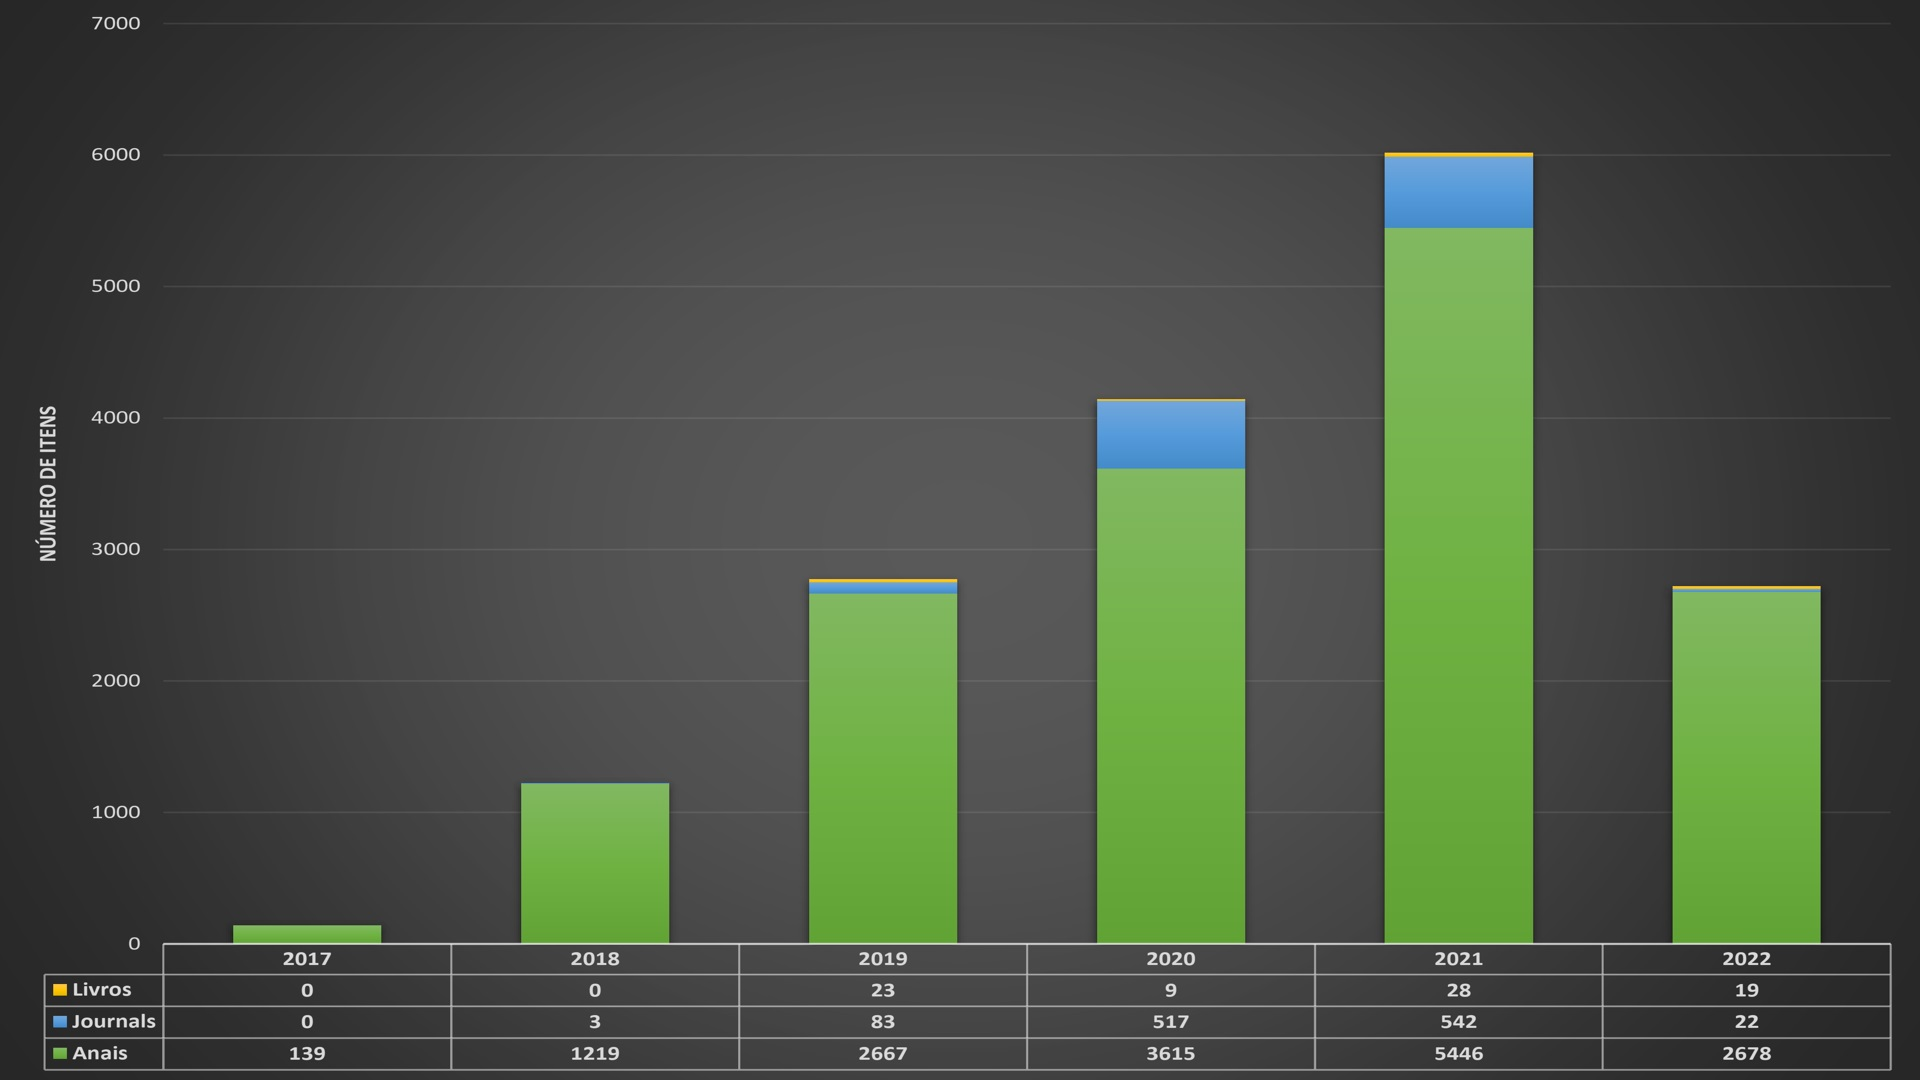
\includegraphics[width=\columnwidth]{sol.jpg}
\caption{Exemplo de legenda de figura.}\label{Fig1}
\end{center}
\end{figure}

Lorem ipsum dolor sit amet, consectetur adipiscing elit, sed do eiusmod tempor incididunt ut labore et dolore magna aliqua. Ut enim ad minim veniam, quis nostrud exercitation ullamco laboris nisi ut aliquip ex ea commodo consequat. Duis aute irure dolor in reprehenderit in voluptate velit esse cillum dolore eu fugiat nulla pariatur. Excepteur sint occaecat cupidatat non proident, sunt in culpa qui officia deserunt mollit anim id est laborum. Lorem ipsum dolor sit amet, consectetur adipiscing elit, sed do eiusmod tempor incididunt ut labore et dolore magna aliqua. Ut enim ad minim veniam, quis nostrud exercitation ullamco laboris nisi ut aliquip ex ea commodo consequat. Duis aute irure dolor in reprehenderit in voluptate velit esse cillum dolore eu fugiat nulla pariatur. Excepteur sint occaecat cupidatat non proident, sunt in culpa qui officia deserunt mollit anim id est laborum.

Lorem ipsum dolor sit amet, consectetur adipiscing elit, sed do eiusmod tempor incididunt ut labore et dolore magna aliqua. Ut enim ad minim veniam, quis nostrud exercitation ullamco laboris nisi ut aliquip ex ea commodo consequat. Duis aute irure dolor in reprehenderit in voluptate velit esse cillum dolore eu fugiat nulla pariatur. Excepteur sint occaecat cupidatat non proident, sunt in culpa qui officia deserunt mollit anim id est laborum. Lorem ipsum dolor sit amet, consectetur adipiscing elit, sed do eiusmod tempor incididunt ut labore et dolore magna aliqua. Ut enim ad minim veniam, quis nostrud exercitation ullamco laboris nisi ut aliquip ex ea commodo consequat. Duis aute irure dolor in reprehenderit in voluptate velit esse cillum dolore eu fugiat nulla pariatur. Excepteur sint occaecat cupidatat non proident, sunt in culpa qui officia deserunt mollit anim id est laborum \textbf{Figure \ref{Fig2}}.

\begin{figure*}
\begin{center}
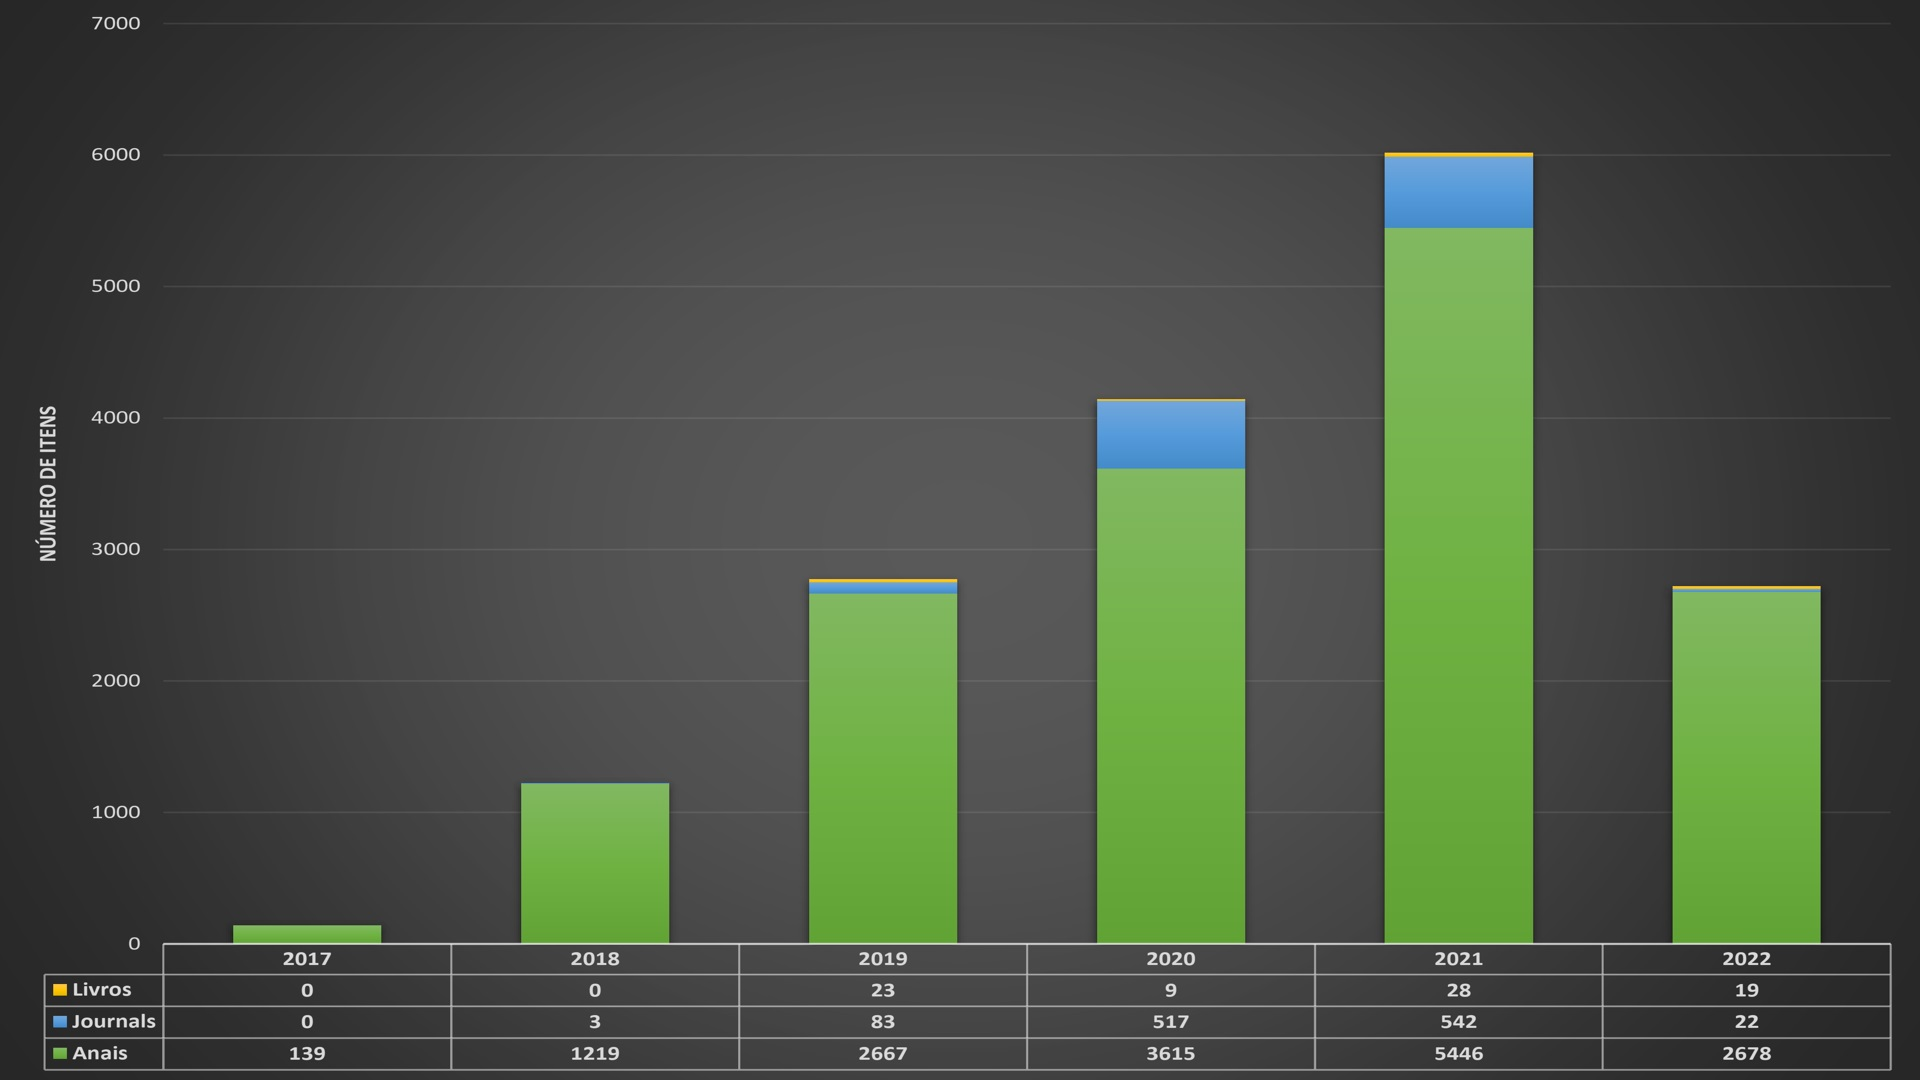
\includegraphics[width=30pc]{sol.jpg}
\caption{{Exemplo de legenda de figura.}}
 \label{Fig2}
\end{center}
\end{figure*}

Lorem ipsum dolor sit amet, consectetur adipiscing elit, sed do eiusmod tempor incididunt ut labore et dolore magna aliqua. Ut enim ad minim veniam, quis nostrud exercitation ullamco laboris nisi ut aliquip ex ea commodo consequat. Duis aute irure dolor in reprehenderit in voluptate velit esse cillum dolore eu fugiat nulla pariatur. Excepteur sint occaecat cupidatat non proident, sunt in culpa qui officia deserunt mollit anim id est laborum. Lorem ipsum dolor sit amet, consectetur adipiscing elit, sed do eiusmod tempor incididunt ut labore et dolore magna aliqua. Ut enim ad minim veniam, quis nostrud exercitation ullamco laboris nisi ut aliquip ex ea commodo consequat. Duis aute irure dolor in reprehenderit in voluptate velit esse cillum dolore eu fugiat nulla pariatur. Excepteur sint occaecat cupidatat non proident, sunt in culpa qui officia deserunt mollit anim id est laborum.

Lorem ipsum dolor sit amet, consectetur adipiscing elit, sed do eiusmod tempor incididunt ut labore et dolore magna aliqua. Ut enim ad minim veniam, quis nostrud exercitation ullamco laboris nisi ut aliquip ex ea commodo consequat. Duis aute irure dolor in reprehenderit in voluptate velit esse cillum dolore eu fugiat nulla pariatur. Excepteur sint occaecat cupidatat non proident, sunt in culpa qui officia deserunt mollit anim id est laborum. Lorem ipsum dolor sit amet, consectetur adipiscing elit, sed do eiusmod tempor incididunt ut labore et dolore magna aliqua. Ut enim ad minim veniam, quis nostrud exercitation ullamco laboris nisi ut aliquip ex ea commodo consequat. Duis aute irure dolor in reprehenderit in voluptate velit esse cillum dolore eu fugiat nulla pariatur. Excepteur sint occaecat cupidatat non proident, sunt in culpa qui officia deserunt mollit anim id est laborum.

Lorem ipsum dolor sit amet, consectetur adipiscing elit, sed do eiusmod tempor incididunt ut labore et dolore magna aliqua. Ut enim ad minim veniam, quis nostrud exercitation ullamco laboris nisi ut aliquip ex ea commodo consequat. Duis aute irure dolor in reprehenderit in voluptate velit esse cillum dolore eu fugiat nulla pariatur. Excepteur sint occaecat cupidatat non proident, sunt in culpa qui officia deserunt mollit anim id est laborum. Lorem ipsum dolor sit amet, consectetur adipiscing elit, sed do eiusmod tempor incididunt ut labore et dolore magna aliqua. Ut enim ad minim veniam, quis nostrud exercitation ullamco laboris nisi ut aliquip ex ea commodo consequat. Duis aute irure dolor in reprehenderit in voluptate velit esse cillum dolore eu fugiat nulla pariatur. Excepteur sint occaecat cupidatat non proident, sunt in culpa qui officia deserunt mollit anim id est laborum.



\paragraph{Exemplo de Título Nível 4.}

Excepteur sint occaecat cupidatat non proident, sunt in culpa qui officia deserunt mollit anim id est laborum. Lorem ipsum dolor sit amet, consectetur adipiscing elit, sed do eiusmod tempor incididunt ut labore et dolore magna aliqua. Ut enim ad minim veniam, quis nostrud exercitation ullamco laboris nisi ut aliquip ex ea commodo consequat. Duis aute irure dolor in reprehenderit in voluptate velit esse cillum dolore eu fugiat nulla pariatur. 

Lorem ipsum dolor sit amet, consectetur adipiscing elit, sed do eiusmod tempor incididunt ut labore et dolore magna aliqua. Ut enim ad minim veniam, quis nostrud exercitation ullamco laboris nisi ut aliquip ex ea commodo consequat. Excepteur sint occaecat cupidatat non proident, sunt in culpa qui officia deserunt mollit anim id est laborum. Lorem ipsum dolor sit amet, consectetur adipiscing elit, sed do eiusmod tempor incididunt ut labore et dolore magna aliqua. Ut enim ad minim veniam, quis nostrud exercitation ullamco laboris nisi ut aliquip ex ea commodo consequat. Duis aute irure dolor in reprehenderit in voluptate velit esse cillum dolore eu fugiat nulla pariatur. Excepteur sint occaecat cupidatat non proident, sunt in culpa qui officia deserunt mollit anim id est laborum.

\section{Conclusão}

Excepteur sint occaecat cupidatat non proident, sunt in culpa qui officia deserunt mollit anim id est laborum. Lorem ipsum dolor sit amet, consectetur adipiscing elit, sed do eiusmod tempor incididunt ut labore et dolore magna aliqua. Ut enim ad minim veniam, quis nostrud exercitation ullamco laboris nisi ut aliquip ex ea commodo consequat. Duis aute irure dolor in reprehenderit in voluptate velit esse cillum dolore eu fugiat nulla pariatur. 

Lorem ipsum dolor sit amet, consectetur adipiscing elit, sed do eiusmod tempor incididunt ut labore et dolore magna aliqua. Ut enim ad minim veniam, quis nostrud exercitation ullamco laboris nisi ut aliquip ex ea commodo consequat. Excepteur sint occaecat cupidatat non proident, sunt in culpa qui officia deserunt mollit anim id est laborum. Lorem ipsum dolor sit amet, consectetur adipiscing elit, sed do eiusmod tempor incididunt ut labore et dolore magna aliqua. Ut enim ad minim veniam, quis nostrud exercitation ullamco laboris nisi ut aliquip ex ea commodo consequat. Duis aute irure dolor in reprehenderit in voluptate velit esse cillum dolore eu fugiat nulla pariatur. Excepteur sint occaecat cupidatat non proident, sunt in culpa qui officia deserunt mollit anim id est laborum \citep{ref5}.


\begin{declarations}

\begin{acknowledgements}
ESTA DECLARAÇÃO É OPCIONAL. Este é um texto de agradecimentos com várias linhas. Lorem ipsum dolor sit amet, consectetur adipiscing elit, sed do eiusmod tempor incididunt ut labore et dolore magna aliqua. Ut enim ad minim veniam, quis nostrud exercitation ullamco laboris nisi ut aliquip ex ea commodo consequat.
\end{acknowledgements}


\begin{funding}
ESTA DECLARAÇÃO É OPCIONAL. Esta pesquisa foi financiada por lorem ipsum dolor sit amet, consectetur adipiscing elit.
\end{funding}

\begin{contributions}
ESTA DECLARAÇÃO É OBRIGATÓRIA. 
\textit{Considerar o Código de Conduta da SBC.
Participação em autoria: espera-se que todos os autores de um trabalho publicado 
ou submetido para publicação, tenham tido efetiva participação no respectivo trabalho.}
Sugerimos que os autores descrevam sua contribuição usando 
a Taxonomia CRediT (\href{https://credit.niso.org/}{https://credit.niso.org/}) como neste exemplo: 
JV contribuiu para a concepção deste estudo. CB, RP e CM realizaram os experimentos. 
JV é o principal contribuidor e escritor deste manuscrito. 
Todos os autores leram e aprovaram o manuscrito final. 
\end{contributions}

\begin{interests}
ESTA DECLARAÇÃO É OBRIGATÓRIA. 
Se não houver conflitos de interesse, os autores devem declarar: 
``Os autores declaram que não têm nenhum conflito de interesses''. 
Caso contrário, a declaração deve ser: 
``Os autores declaram que têm os seguintes conflitos de interesses: 
lorem ipsum dolor sit amet, consectetur adipiscing elit.''
\end{interests}

\begin{materials}
ESTA DECLARAÇÃO É OBRIGATÓRIA. 
\textit{Considerar o Código de Conduta da SBC. 
Reprodutibilidade de resultados de pesquisa: 
nos casos pertinentes, recomenda-se que artigos indiquem 
a disponibilidade pública de material utilizado nas revisões, 
de modo a facilitar a reprodução dos respectivos resultados por outros pesquisadores.}
%
Se os autores disponibilizaram seus dados e/ou códigos abertamente, a declaração deve ser: 
``Os dados e outros materiais criados e/ou usados nesta revisão da literatura
estão disponíveis em \ldots''. 
Caso contrário, a declaração deve ser: 
``Os dados e outros materiais criados e/ou usados nesta revisão da literatura 
serão disponibilizados mediante solicitação''. 
%
Todo o material suplementar disponibilizado publicamente pelos autores aparecerá 
na página de publicação do artigo em caso de aceitação. 
\end{materials}

\begin{aitools}
ESTA DECLARAÇÃO É OBRIGATÓRIA.  
\textit{Considerar o Código de Conduta da SBC.
Uso de Inteligência Artificial (IA) Generativa: 
a utilização de ferramentas e tecnologias de IA Generativa para geração de conteúdos, 
na escrita e/ou revisão do conteúdo de artigos, deve ser declarada explicitamente no trabalho.} 
A declaração deve ocorrer nesta seção, definida especificamente para este fim.
Deve-se listar as ferramentas (e suas versões) e descrever onde foram empregadas, por exemplo, 
textos, tabelas, gráficos, citações, etc. 
Essas ferramentas \textbf{não} podem ser listadas como autores de um artigo. 
O uso de tais ferramentas não exime os autores da responsabilidade 
sobre todo o seu conteúdo, inclusive no caso de ser identificado plágio.
%
Se os autores não utilizaram tais ferramentas, a declaração deve ser: 
``Os autores não utilizaram ferramentas de IA generativa no desenvolvimento do estudo''.
%
\end{aitools}

\begin{furtherinformation}
Manuscritos devem indicar explicitamente como as questões éticas da pesquisa foram abordadas e gerenciadas, 
incluindo a aprovação da pesquisa por um comitê de ética, quando aplicável.
\end{furtherinformation}

\end{declarations}

\bibliographystyle{apalike-sol}
\bibliography{refs}

\end{document}

